\documentclass{article}
\usepackage{enumerate}
\usepackage{amsmath}
\usepackage{amssymb}
\usepackage{graphicx}
\usepackage{subfigure}
\usepackage{geometry}
\usepackage{caption}
\usepackage{indentfirst}

\usepackage{algorithm}  
\usepackage{algorithmicx}  
\usepackage{algpseudocode}
\renewcommand{\algorithmicrequire}{\textbf{Input:}}  
\renewcommand{\algorithmicensure}{\textbf{Output:}}  
\usepackage{minted}
\usemintedstyle{autumn}
\setminted{linenos,breaklines,tabsize=4,xleftmargin=1.5em}

\geometry{left=3.0cm,right=3.0cm,top=3.0cm,bottom=4.0cm}

\title{VE281 Project Three Report}
\author{Liu Yihao 515370910207}
\date{}

\begin{document}
\maketitle

\section{Introduction}

In order to study the performances of these three priority queues, I generated random inputs with different grid sizes and compared the running speed of them (including std::priority\_queue in STL). Since it's a waste of time to wrote a comparison script written in C++, I chose node-gyp to build the sorting algorithm into a C++ addon of node, and then wrote some Javascript code to benchmark them. Small size of arrays were run for several times so that the result can be more accurate.

\section{Comparison of algorithms}

The limitation of runtime was set to 1s for all algorithms, so some meaningless and slow running were dropped. Then I used MATLAB to plot a graph.

\begin{figure}[!htbp]
\centering
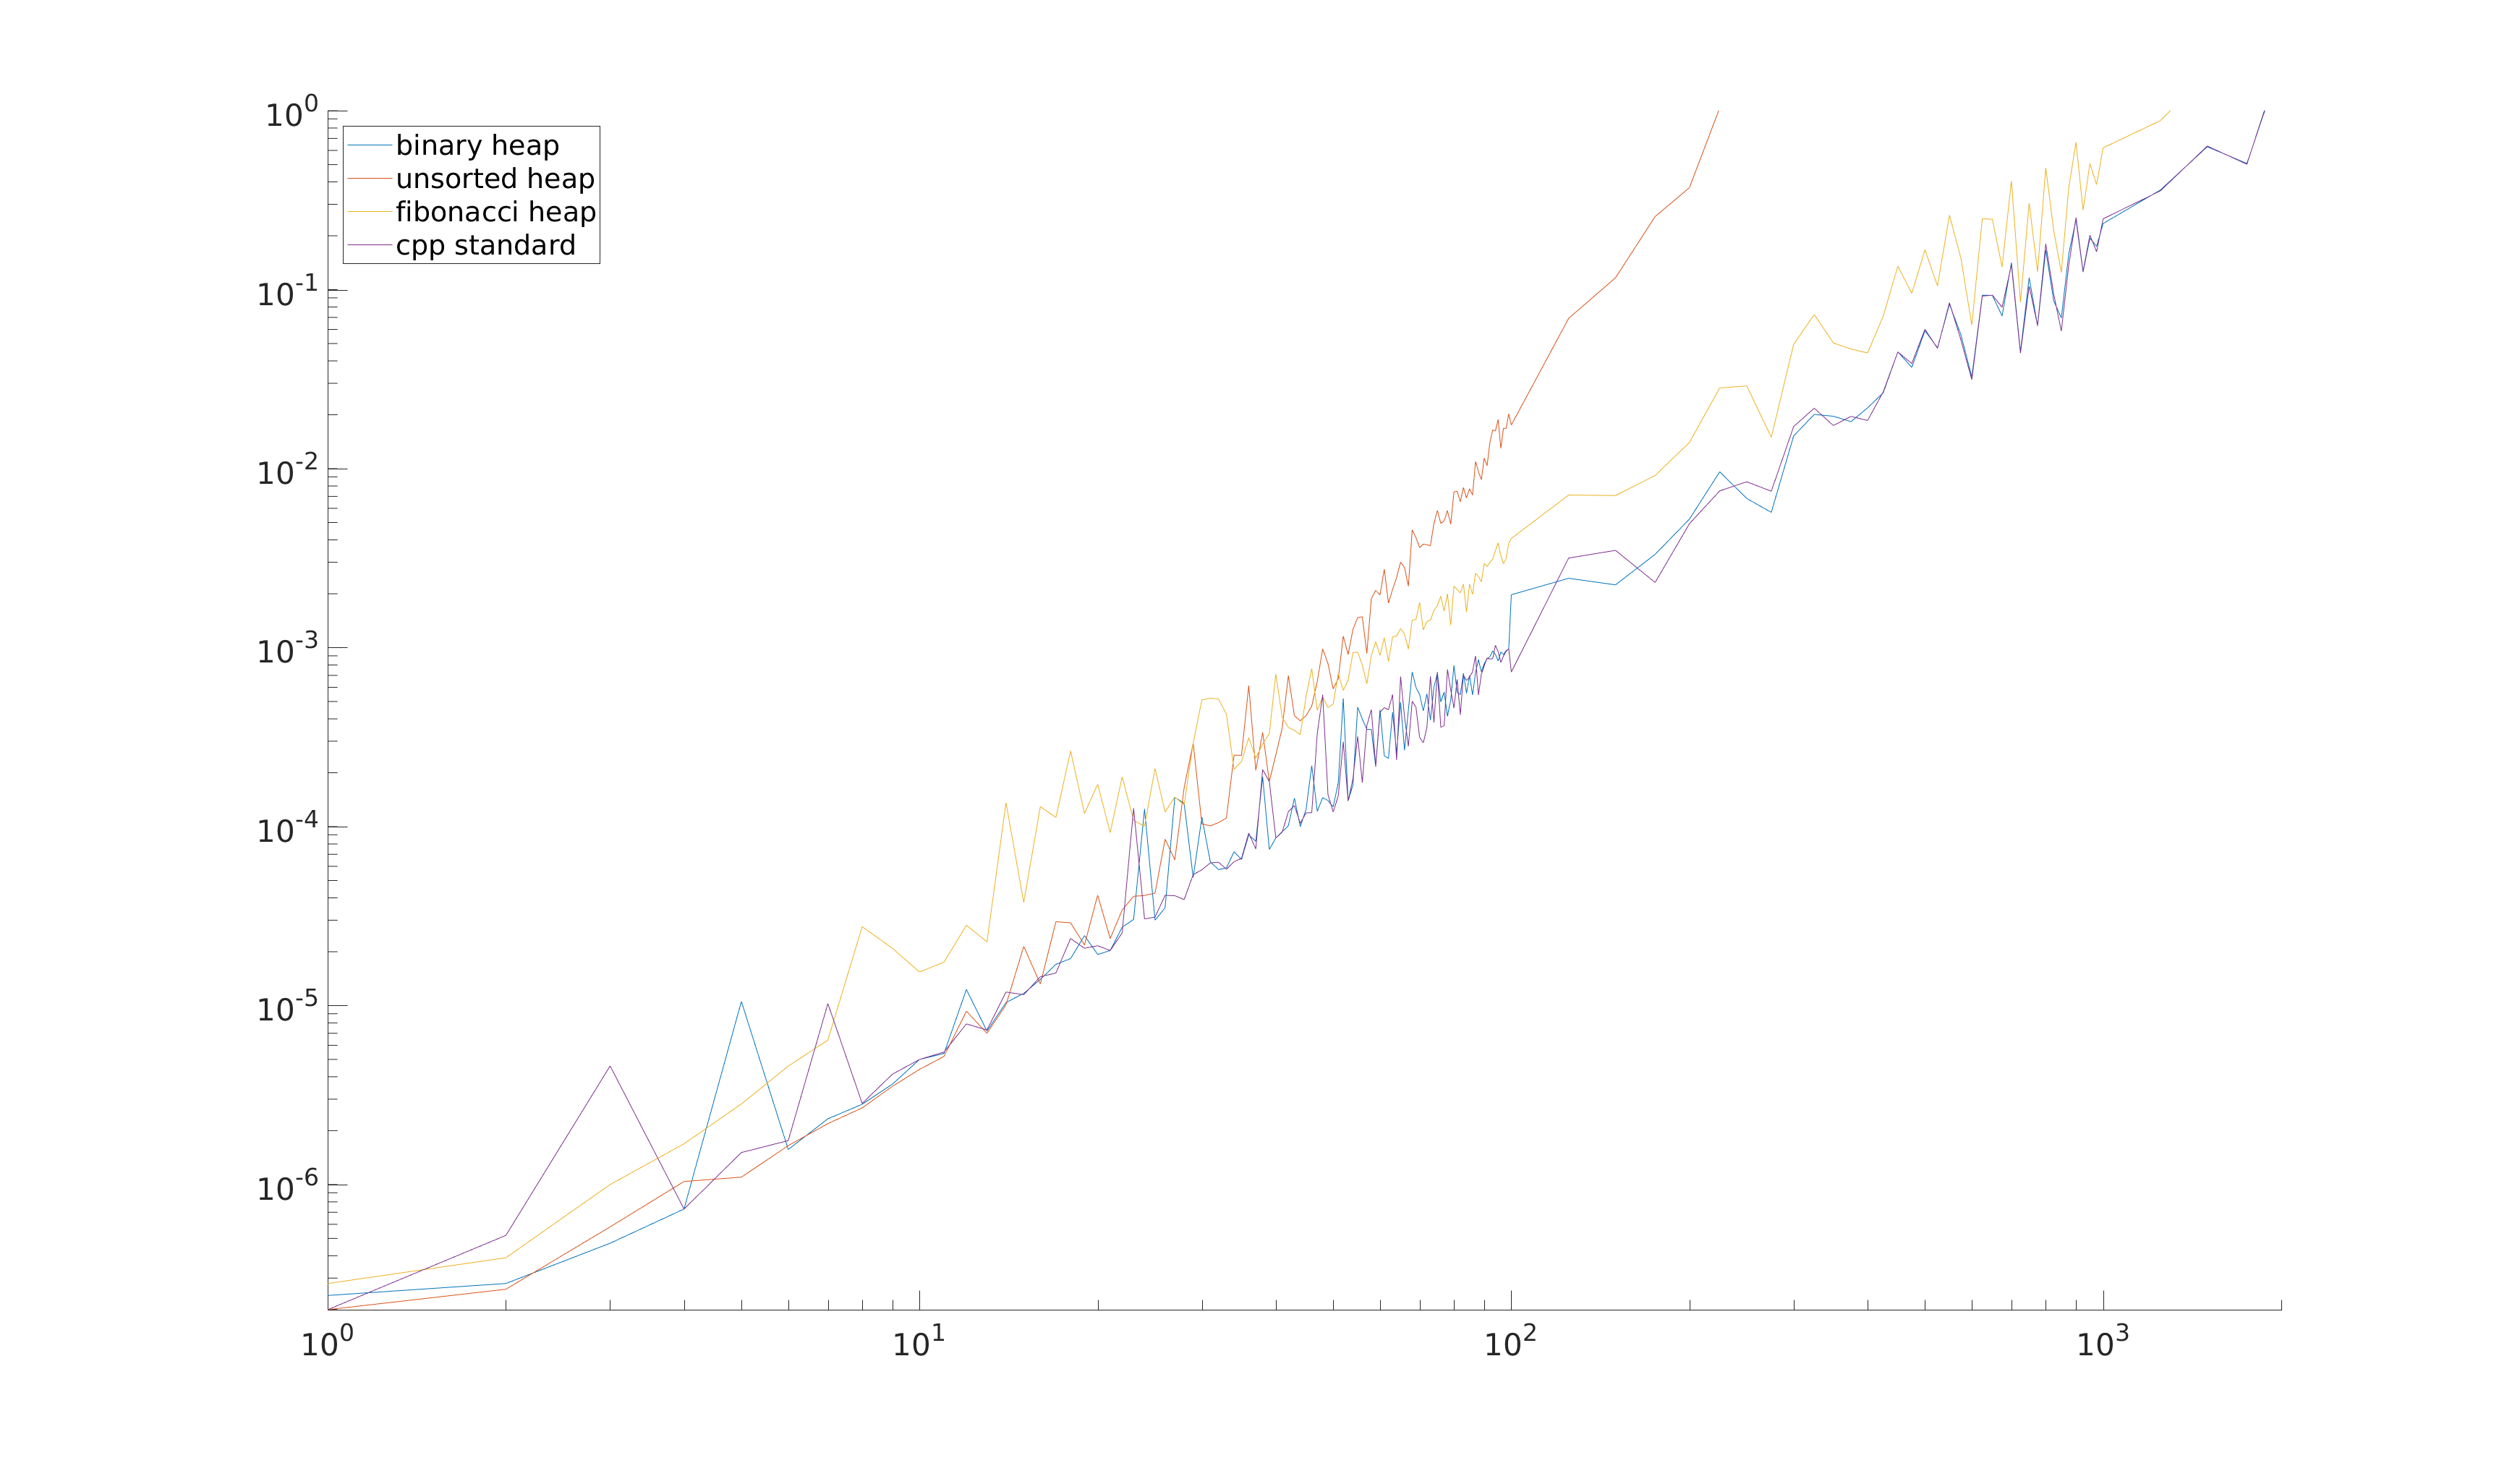
\includegraphics[width=0.8\linewidth]{../benchmark/fig1.png}
\caption{All cases}
\label{fig-1}
\end{figure}

From Figure \ref{fig-1}, we can find that binary\_heap, fib\_heap and std::priority\_queue have the similar running speed. The result satisfy the theory that they have the time complexity of $O(\log n)$ in enqueing, finding minimum and dequeing minimum. However, unsorted\_heap is slower than those three queues, because it have the time complexity of $O(n)$ in finding minimum and dequeing minimum. 

\newpage

\section{Appendix}

\subsection{The project files}

\subsubsection{binary\_heap.h}
\inputminted{c++}{../answer/binary_heap.h}
\subsubsection{unsorted\_heap.h}
\inputminted{c++}{../answer/unsorted_heap.h}
\subsubsection{fib\_heap.h}
\inputminted{c++}{../answer/fib_heap.h}
\subsubsection{main.cpp}
\inputminted{c++}{../answer/main.cpp}
\subsubsection{Makefile}
\inputminted{makefile}{../answer/Makefile}


\subsection{The benchmark program}
\subsubsection{README.md}
\inputminted{md}{../benchmark/README.md}
\subsubsection{queue\_wrapper.h}
\inputminted{c++}{../benchmark/queue_wrapper.h}
\subsubsection{queue\_wrapper.cpp}
\inputminted{c++}{../benchmark/queue_wrapper.cpp}
\subsubsection{binding.gyp}
\inputminted{json}{../benchmark/binding.gyp}
\subsubsection{benchmark.js}
\inputminted{javascript}{../benchmark/benchmark.js}
\subsubsection{benchmark.m}
\inputminted{matlab}{../benchmark/benchmark.m}

\end{document}
